Per identificare le stelle in cielo sono state divise in costellazioni, le quali sono una appartenenza ad un gruppo di stelle legato alla visualizzazione di figure (Cefeo, Orsa Maggiore, Orione ecc...), tale metodo vale però per le stelle molto luminose e richiede una conoscenza molto generale.

\E preferibile però identificare le stelle in un quadrante di cielo molto piccolo, in modo da identificare singolarmente ogni stella. Per fare ciò serve un sistema di riferimento. Il sistema di riferimento naturale è quello in cui il piano in cui ci troviamo diventa il nostro orizzonte, dove abbiamo le 4 direzioni Nord, Sud, Est ed Ovest; in tale sistema vi è inoltre un punto privilegiato chiamato \textbf{zenith}, posto sopra di noi. Gli oggetti appaiono sulla sfera celeste\footnote{La sfera celeste è una sfera immaginaria, di raggio arbitrario e con al centro la Terra, sulla cui superficie si proiettano tutti gli astri. La sfera celeste non ha nessuna realtà fisica, è solo un'illusione dovuta al fatto che non siamo in grado di valutare visivamente la diversa distanza dei corpi celesti.} e possiamo pensare di identificare la posizione di un oggetto tramite le coordinate sferiche (in particolare ci bastano gli angoli). Per convenzione, come direzione privilegiata si è scelto il cerchio massimo passante per lo zenith e la Polare, il quale è detto \textbf{meridiano principale}, che noi chiamiamo Sud (se guardiamo in direzione opposta alla polare sul cerchio massimo guardiamo il Sud, cioè dove culmina il Sole a mezzogiorno).

\begin{minipage}{0.295\textwidth}
    \begin{figure}[H]
        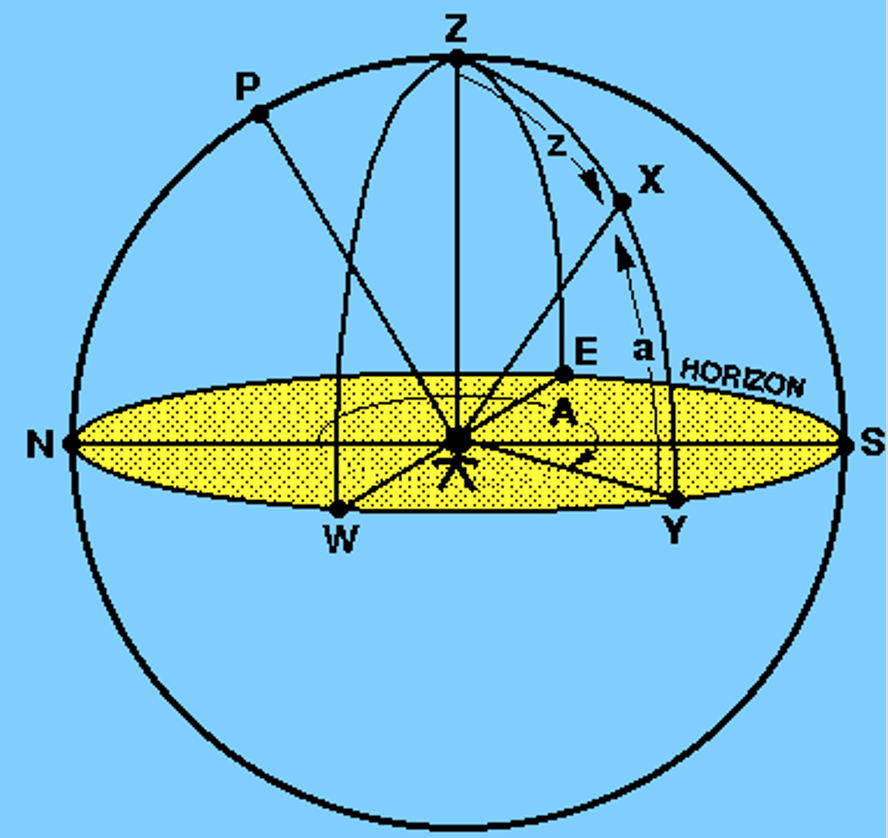
\includegraphics[width=5 cm]{immagini/coordinate_altazimutali.png}
    \end{figure}
\end{minipage}
\begin{minipage}{0.7\textwidth}
    \hspace{0.6cm}\vspace{-0.3cm}Definiamo le \textbf{coordinate altazimutali}:
    \vspace{0.3cm}
    \begin{itemize}
        \item \textbf{Altezza:} distanza angolare dell'oggetto dall'orizzonte.
        \item \textbf{Azimut:} distanza angolare tra il meridiano passante per la stella e il meridiano principale.
    \end{itemize}
    \hspace{0.6cm}Possiamo definire analogamente la \textbf{distanza zenitale} 
    
    \hspace{0.6cm}come la distanza angolare dell'oggetto dallo zenith.
\end{minipage}

Il problema di questo sistema di riferimento è che esso cambia in base alla posizione dell'osservatore. Per esempio al polo Nord la polare ha una altezza di $90^\circ$, mentre all'equatore la polare si trova sull'orizzonte, per cui ha un'altezza di $0^\circ$.

%\begin{figure}[ht]
%    \centering
%    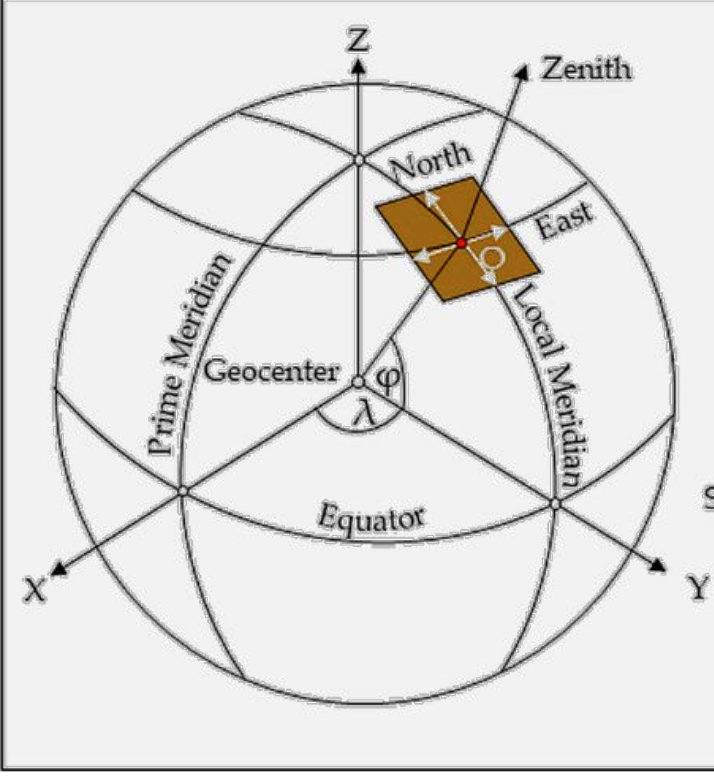
\includegraphics[width=5 cm]{Piano dell'orizzonte sulla terra.png}
%\end{figure}

Inoltre durante lo scorrere del tempo gli oggetti si muovono di 15 gradi all'ora, quindi azimut e altezza cambiano continuamente. Tale sistema è dunque inutilizzabile.

Per avere un sistema di riferimento comune, poniamo l'orizzonte coincidente con l'equatore rotazionale terrestre, che è comune a tutti, e definiamo un meridiano fondamentale. A questo punto chiamiamo \textbf{declinazione} l'altezza in angoli dell'oggetto sull'orizzonte; la chiamiamo così perché è una proprietà dell'oggetto, non più dell'osservatore. Siccome le stelle sono ferme (è la Terra che ruota), con una opportuna convenzione il nuovo azimut è un \textbf{angolo orario} $H$ che cambierà con il ruotare della Terra, quindi dipenderà dall'ora del luogo.

\begin{minipage}{0.345\textwidth}
    \begin{figure}[H]
        \centering
        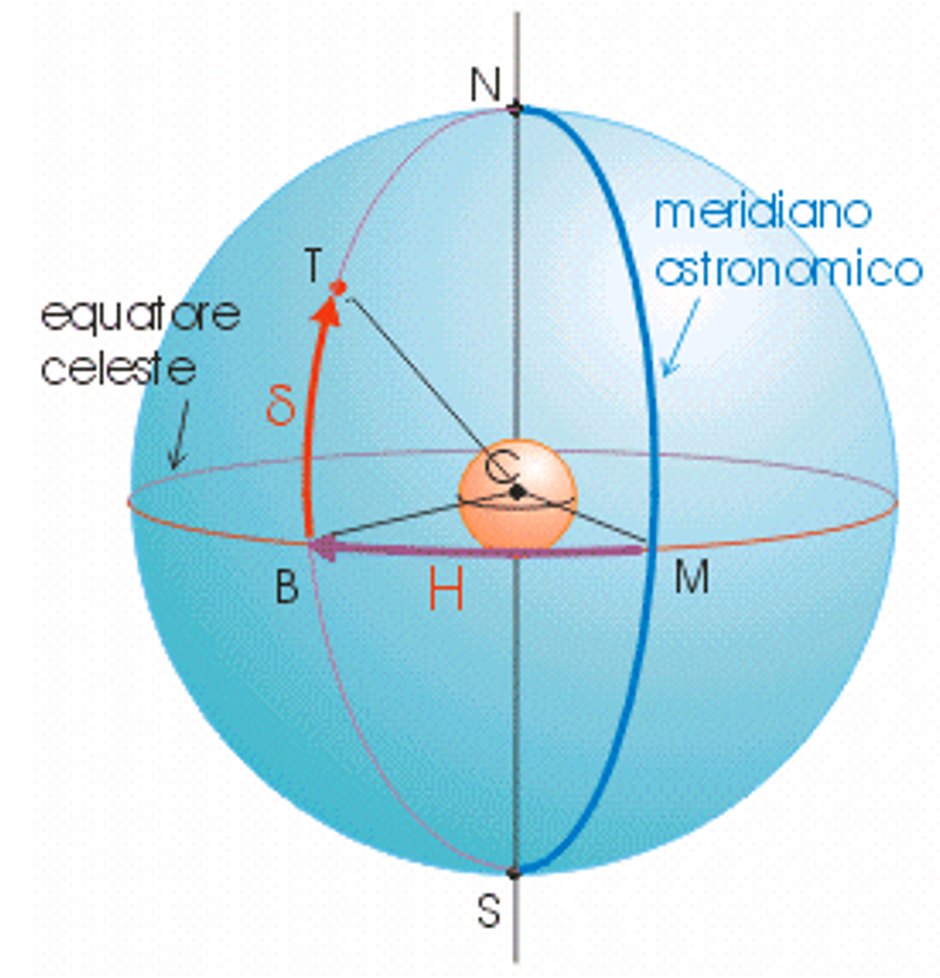
\includegraphics[width=5 cm]{Coordinate orarie.png}
    \end{figure}
\end{minipage}
\begin{minipage}{0.65\textwidth}
    \vspace{0.5cm}Ad esempio, se una stella si trova sul meridiano di Greenwich, che per noi rappresenta il meridiano di riferimento, ha angolo orario 0; per noi che siamo a Catania ha angolo orario 1.

    Se sappiamo dove siamo localizzati come time-zone possiamo conoscere l'angolo orario e puntare lo stesso oggetto: basterà sommare il fuso orario all'angolo orario. In questo modo l'angolo orario diventa una coordinata insieme alla declinazione tale da essere indipendente dal posto in cui si trova l'osservatore.
\end{minipage}

\vspace{0.2cm}Tuttavia si ha ancora uno svantaggio: la Terra ruota intorno al Sole. Un sistema migliore sarebbe allora un sistema esterno ma ancora solidale con la Terra, dove l'angolo orario non sia legato a Greenwich. Potremmo ad esempio trovare un riferimento per conteggiare gli angoli legato alla posizione occupata dal Sole in un determinato periodo dell'anno.

\begin{minipage}{0.345\textwidth}
    \begin{figure}[H]
        \centering
        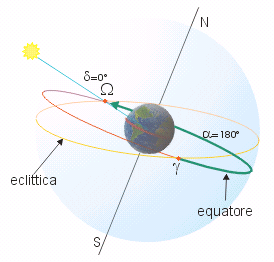
\includegraphics[width=5 cm]{immagini/coordinate_equatoriali.png}
    \end{figure}
\end{minipage}
\begin{minipage}{0.65\textwidth}
    \vspace{0.3cm}Durante l'anno il Sole compie un moto apparente che porta a farlo apparire più in alto o più in basso rispetto all'orizzonte; ad un certo punto occuperà due punti chiamati \textbf{nodi}, i quali rappresentano l'intersezione del piano equatoriale con il piano orbitale\footnotemark. Il punto che occupa passando da declinazioni negative a declinazioni positive (ciò avviene in primavera) è detto punto $\gamma$, quello che occupa passando declinazioni positive a declinazioni negative è detto punto $\Omega$ (ciò avviene in autunno).
\end{minipage}

\footnotetext{\E chiaro che l'intersezione di due piani è una retta: la \textit{linea dei nodi}. Per essere precisi i nodi sono l'intersezione tra l'orbita e un piano di riferimento, come ad esempio quello equatoriale.}

\vspace{0.3cm}Si può allora pensare di dare alle stelle una coordinata rispetto ad un punto fisso nel cielo, che è il nodo. Chiamiamo dunque \textbf{ascensione retta} $\alpha$ l'angolo fra la posizione della stella e il punto $\gamma$ nel piano equatoriale. Essa diventa una misura oggettiva della posizione angolare, in quanto non dipende dal luogo e dall'orario.

\vspace{0.2cm}Dobbiamo sapere però come passare dalle coordinate equatoriali a quelle altazimutali. Abbiamo definito l'angolo orario come la distanza angolare rispetto al meridiano Greenwich, adesso ci chiediamo qual è l'angolo orario fra il punto $\gamma$ e il meridiano di Greenwich. Si definisce pertanto il \textbf{tempo siderale} $ST$ come l'ascensione retta degli oggetti che stanno al meridiano. Tramite questo l'angolo orario sarà dato

$$H=ST-\alpha$$

In questo modo risulta facile capire dove puntare il telescopio.

Tramite l'ascensione retta e la declinazione si possono creare delle mappe del cielo.

\vspace{0.2cm}Tutto questo si basa sull'inclinazione dell'asse terrestre rispetto al piano orbitale che nelle considerazioni precedenti abbiamo supposto rimanere costante, ma non è così:

\vspace{-0.3cm}

\begin{minipage}{0.345\textwidth}
    \begin{figure}[H]
        \centering
        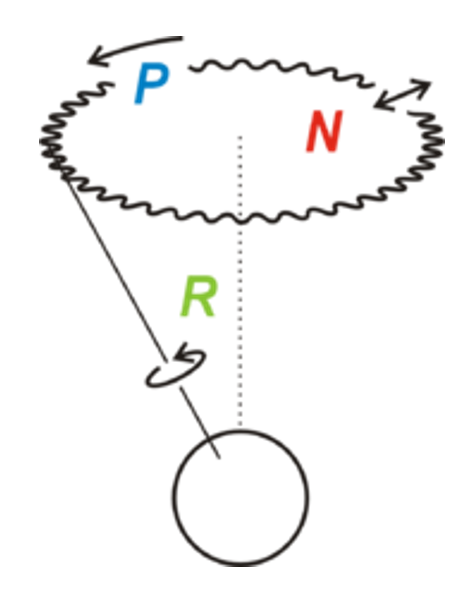
\includegraphics[width=4cm]{immagini/precessione_e_nutazione.png}
    \end{figure}
\end{minipage}
\begin{minipage}{0.65\textwidth}
    \vspace{0.5cm}La Terra, similmente ad una trottola, compie un moto di precessione\footnotemark. Il periodo di \textbf{precessione} dura 25772 anni, che è molto lungo rispetto ai tempi umani, per cui diventa un fattore incisivo solo se si vuole una grande precisione.

    A questo effetto di precessione inoltre, si somma il movimento di \textbf{nutazione} dovuto alla presenza della Luna. A causa di questi effetti, l'asse di rotazione la Terra descrive la figura mostrata nell'immagine.
\end{minipage}

\footnotetext{La precessione è il cambiamento della direzione dell'asse di rotazione di un corpo in movimento rotatorio.}

Il periodo di precessione è troppo lungo per essere ignorato? Numericamente si ha che

$$\frac{2\pi}{25772\ yr}=\frac{2\pi}{25772\cdot 365.25\ d}=6.67\cdot 10^{-7}\ \text{rad/day}$$

cioè le stelle si spostano ogni giorno di $6.67\cdot 10^{-7}$ radianti.

In astronomia però radianti e gradi sono troppo grandi, si preferisce utilizzare delle unità di misura legate al tempo. In particolare si usano gli arcominuti $[']$ e gli arcosecondi $['']$.

$$1\text{ arcmin}=\frac{1^\circ}{60}\qquad 1 \arcsec =\frac{1'}{60}=\frac{1^\circ}{3600}$$

Convertiamo gli arcosecondi in radianti

$$1 \arcsec =\frac{1^\circ}{3600}=\frac{2\pi}{360\cdot3600}=4.848137\cdot 10^{-6}\ \text{rad}$$

Quindi

$$1\text{rad}=206264.8062''$$

Per dare una idea di quanto valga un arcosecondo, una stella a livello del mare è grande $5''$, in montagna $2''$\textbf{non sono sicuro sulla nota}\footnote{Il motivo di questa differenza è dovuta alla rifrazione dell'atmosfera.}.

La precessione in arcosecondi è di $0.13''$ al giorno. Ne segue che bisogna tener conto della precessione, altrimenti rischieremmo di sbagliare a puntare se volessimo osservare una stella più volte a distanza di tempo.

Un altro effetto di cui tenere conto è il fatto che l'atmosfera terrestre fa rifrangere la luce, quindi gli oggetti cambiano di posizione. In particolare la rifrazione dipende dalla distanza zenitale.

Esiste un sistema di riferimento internazionale centrato nel Sole e i cui tre assi sono definiti con gli oggetti più lontani che conosciamo (perché si suppone che più un oggetto è lontano meno lo vedremo muovere, cioè la distanza apparente è minore). Il sistema di riferimento è chiamato \textbf{International Celestial Reference System} (ICRS) è stato deciso dalla International Astronomical Union (IAU). Abbiamo cataloghi con migliaia di oggetti con le loro coordinate. Il database più grande si trova sul sito \textit{simbad}.